% lang_pack — Language Pack Manual (covtl-pipeline)
% SPDX-FileCopyrightText: 2026 Frédéric Berthommier
% SPDX-License-Identifier: GPL-3.0-or-later
%
% Compile with plain pdflatex (standard packages only):
%     pdflatex manual.tex && pdflatex manual.tex
% (run twice for the table of contents and cross references)

\documentclass[11pt,a4paper]{article}

\usepackage[T1]{fontenc}
\usepackage[utf8]{inputenc}
\usepackage{lmodern}
\usepackage[margin=2.5cm]{geometry}
\usepackage{amsmath}
\usepackage{amssymb}
\usepackage{graphicx}
\usepackage{booktabs}
\usepackage{longtable}
\usepackage{xcolor}
\usepackage[colorlinks=true, linkcolor=blue!55!black,
            urlcolor=blue!55!black]{hyperref}

\setlength{\parindent}{0pt}
\setlength{\parskip}{0.45em}

\newcommand{\code}[1]{\texttt{#1}}
\newcommand{\sampkey}[1]{\texttt{#1}}

\title{\textbf{The covtl-pipeline Language Pack}\\[0.4em]
\large Installing and calibrating six synthesis languages\\
(English, French, Spanish, German, Italian, Portuguese)}
\author{Fr\'ed\'eric Berthommier}
\date{Version 1.1.0 --- September 2026}

\begin{document}

\noindent\textbf{\color{red} v1.0.9 update --- parts of this manual superseded.} Since v1.0.9 (2026-09-23) the LANG SECTION is a \emph{marker only} (\code{ACTIVE\_LANG}): the language pack no longer installs per-language vowel targets, the JD3 guard is removed (defect D24 resolved), and \code{calibrate} is deprecated. Vowel targets and effort gains are the \emph{active speaker’s own}; they were recalibrated per speaker in v1.0.9 (see \code{docs/SPEAKERS.md}). The sections below that describe per-language targets, the guard, and the calibration commands describe the pre-1.0.9 behaviour.


\maketitle

\begin{center}
\begin{minipage}{0.86\textwidth}
\small\emph{Scope.} This manual documents the \emph{installable
language package} of the covtl-pipeline articulatory synthesizer: what
it contains, how to install and activate a language, how the vowel
targets are calibrated on the engine (VTL/JD3), and how to extend the
pack with a new language. The engine itself (the Berthommier COVTL
model, VocalTractLab synthesis, the JD3 speaker) is documented in the
main repository manual (\code{docs/manual.pdf}); the
multi-speaker registry is documented in \code{docs/speakers.pdf} and
the expressive-prosody option in
\code{docs/expressive\_prosody.pdf}.
\end{minipage}
\end{center}

\vspace{0.5em}
\tableofcontents
\vspace{1em}

% ===========================================================================
\section{Introduction}
% ===========================================================================

\subsection{What the language pack is}

The covtl-pipeline synthesizes speech by driving the VocalTractLab
(VTL) articulatory synthesizer with trajectories computed by the
Berthommier COVTL model. Originally the pipeline spoke English only
(through the CMUdict grapheme-to-phoneme dictionary). The language
pack extends it to six languages:

\begin{itemize}
\item \textbf{en} --- English (CMUdict; the original pipeline
      calibration, covered by the regression baselines);
\item \textbf{fr} --- French (Wikipron lexicon + rules; LPC-calibrated
      vowel targets, validated in situ);
\item \textbf{es} --- Spanish, Castilian with \emph{distinci\'on}
      (Wikipron \code{spa\_latn\_ca});
\item \textbf{de} --- German (Wikipron; tense/lax vowel pairs,
      final devoicing, \emph{ach/ich}-laut);
\item \textbf{it} --- Italian (Wikipron; no phonological schwa ---
      Tuscan \code{@} is mapped to \sampkey{e});
\item \textbf{pt} --- European Portuguese (Wikipron
      \code{por\_latn\_po}; nasal vowels through the engine
      \sampkey{\textasciitilde} convention).
\end{itemize}

The pack is a \emph{source package}: a directory
(\code{lang\_pack/}) at the repository root that the command
\code{python setup\_lang.py install} copies into the pipeline tree.
Nothing is installed into \code{vtl\_binaries/}, and the JD3 speaker
is \textbf{never} modified.

\subsection{Package layout}

{\small
\begin{verbatim}
lang_pack/
|-- profiles/          g2p + language + expressive profiles -> vtl_synth/utils/
|-- lexicons/          Wikipron TSV + license notices    -> vtl_synth/data/
|-- lang_blocks/       per-language LANG SECTION fragments (blocks.py)
|-- integration/       patched pipeline.py / utils__init__.py
|-- manual/            this manual + figures
|-- install_lang.bat   one-command installer (Windows)
|-- install_lang.sh    one-command installer (Linux/macOS)
|-- README.md          presentation, expected verify scores
|-- LICENSE.md         per-component licensing (GPL-3.0+ / CC BY-SA 3.0)
`-- ARCHITECTURE.md    origins and data flow of every component
\end{verbatim}
}

\subsection{Prerequisites}

\begin{itemize}
\item \textbf{Python $\geq$ 3.9} with \code{numpy} ($\geq$1.22),
      \code{scipy} ($\geq$1.7), \code{cmudict}, and the VTL bindings
      \code{vocaltractlab-cython} ($\geq$0.0.10);
      \code{Pillow} and \code{imageio-ffmpeg} for the video output.
\item The \textbf{JD3 speaker} file in
      \code{vtl\_synth/data/vtl\_binaries/} (shipped with the
      repository --- the pack does not ship and never touches it).
\item The VTL binaries (VocalTractLab~2.3/2.4) reachable by the
      Python bindings.
\item A covtl-pipeline clone with the \code{vtl\_synth} package
      importable (for a local checkout, \code{pip install -e .} from
      the repository root; the Windows installer does it for you).
\end{itemize}

The pronunciation lexicons (\code{lexicons/*.tsv}, about 13~MB
total) ship with the pack; Section~\ref{sec:newlang} gives the exact
download commands if you prefer to fetch them from Wikipron directly.

% ===========================================================================
\section{Quick start}
% ===========================================================================

\subsection{One command on Windows}

Run \code{lang\_pack\textbackslash install\_lang.bat} with the
language code as argument (default \code{fr}):

\begin{verbatim}
    lang_pack\install_lang.bat fr
    lang_pack\install_lang.bat es
\end{verbatim}

The batch locates Python (\code{py -3} or \code{python}), installs
the Python dependencies and the pipeline if needed, then chains the
three pipeline commands:

\begin{verbatim}
    python setup_lang.py install --lang fr
    python setup_lang.py verify
    python setup_lang.py show
\end{verbatim}

At the end you see the active language and the in-situ vowel report.
On Linux/macOS, \code{bash lang\_pack/install\_lang.sh fr} does the
same.

\subsection{The three commands by hand}

\begin{verbatim}
    python setup_lang.py install --lang fr   # install + activate fr
    python setup_lang.py verify              # in-situ LPC proof
    python setup_lang.py show                # current language
\end{verbatim}

\code{install} is idempotent: re-running it refreshes the installed
modules and rewrites the managed language section of
\code{vtl\_synth/core/constants.py}. Every command of
\code{setup\_lang.py} prints the currently active language, so a
terminal always tells you which language the engine is set to.

Switching language after installation is one command and fully
reversible (byte-identical round trip):

\begin{verbatim}
    python setup_lang.py setlang en|fr|es|de|it|pt
    python setup_lang.py list                 # available languages
    python setup_lang.py restore --purge      # full uninstall
\end{verbatim}

\subsection{Installing the whole pack step by step}

\begin{enumerate}
\item Check the prerequisites (Section~1.3).
\item If a lexicon TSV is missing, download it (curl) or copy it from
      \code{lang\_pack/lexicons/} --- see
      \code{lexicons/README\_xx\_lexicon.md} per language. The g2p
      also works without lexicons (rules + exceptions only), with a
      warning.
\item \code{python setup\_lang.py install --lang <xx>}
      --- copies the language profile modules into
      \code{vtl\_synth/utils/}, the lexicons into
      \code{vtl\_synth/data/}, integrates the language-aware
      \code{Pipeline} (the original files are backed up once as
      \code{.bak}), and rewrites the LANG~SECTION of
      \code{constants.py} for the requested language.
\item \code{python setup\_lang.py setlang <xx>} whenever you want
      another language.
\item \code{python setup\_lang.py verify} --- the proof (below).
\item To roll everything back:
      \code{python setup\_lang.py restore --purge} restores the
      pristine pipeline files and removes the installed language
      modules. Repository-tracked lexicons and user-modified data
      files are never deleted.
\end{enumerate}

\begin{figure}[htbp]
\centering
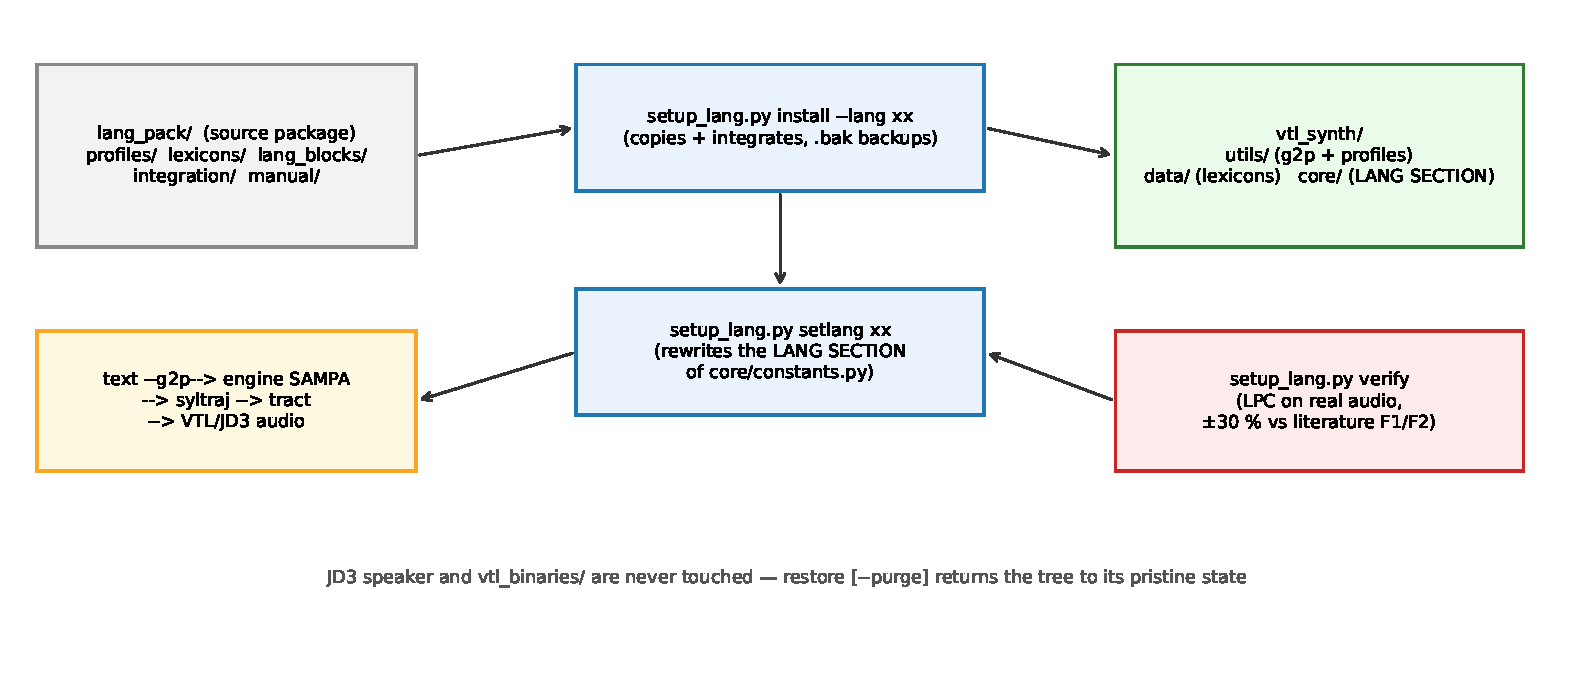
\includegraphics[width=\textwidth]{figures/pipeline_flow.pdf}
\caption{Installation and switching data flow. The pack is the
\emph{source}; \code{install} copies/integrates it into the pipeline
tree; \code{setlang} rewrites the managed LANG~SECTION; \code{verify}
closes the loop by measuring what the engine actually synthesizes.
The JD3 speaker and \code{vtl\_binaries/} are never touched.}
\label{fig:flow}
\end{figure}

\subsection{Reading the verify report}
\label{sec:verify}

\code{verify} is the in-situ proof that the installed vowel targets
produce the intended vowels on \emph{your} engine: for every vowel of
the active language it synthesizes the isolated vowel through the real
pipeline (SAMPA direct, JD3), measures F1/F2 by LPC on the produced
audio, and compares them with the language's reference formants
(literature values for a male speaker of the language; sources
listed in Section~\ref{sec:license}).

\begin{verbatim}
    voy    F1 mes    F1 ref |   F2 mes    F2 ref | verdict
    e          300       400 |      1707      1900 | OK
    o          323       450 |       993       830 | OK
    ...
    [setup_lang] Bilan : 6/7 voyelles dans la tolerance +-30%
\end{verbatim}

A vowel is \emph{OK} when both measured formants are within
$\pm30\%$ of the reference. Compare your \code{Bilan} line with the
expected scores (Table~\ref{tab:verdicts}): a healthy installation
reproduces them (up to $\pm1$ verdict of LPC jitter). A score far
below the published one (e.g.\ 2/7 for Spanish) indicates a broken
installation --- typically missing VTL bindings or a corrupted
constants section --- not a calibration problem.

\begin{table}[htbp]
\centering
\caption{Expected \code{verify} scores ($\pm30\%$ tolerance, JD3),
of the shipped blocks. \emph{fr}: the ``validated'' block
measures 4/12 under the current chain (see the LPC bias below).
\emph{en}: covered by the regression baselines rather than by the
LPC chain (its targets predate the verification tool).}
\label{tab:verdicts}
\begin{tabular}{lll}
\toprule
language & expected \code{Bilan} & notes \\
\midrule
en & 4/8 (measured) & original calibration; formally covered by the
regression baselines \\
fr & 4/12 & documented LPC-measurement gap (see the LPC bias below) \\
es & 6/7 & /i/ F2 ceiling of the engine ($\approx$1300 Hz) \\
de & 10/14 & lax + front-rounded vowels: F1 measured low \\
it & 4/7 & F1 bias on close vowels; /o/ engine limit \\
pt & 5/8 & /o u/ at the tolerance edge (hypotheses) \\
\bottomrule
\end{tabular}
\end{table}

\textbf{The documented LPC bias.} The linear-prediction analysis
chain (11~kHz, pre-emphasis, order 16) systematically measures
\emph{F1 too low on close and rounded vowels} (e.g.\ French /i/: 210
Hz measured vs 280 expected) and is occasionally unstable between
runs on front-rounded vowels and the German schwa (F2 of /@/: 1484
then 896~Hz at an identical target). These deviations are
\emph{measurement} artifacts, documented per vowel in the comments of
the language blocks --- they are not installation errors. The
per-vowel comments next to each target in \code{constants.py} carry
the measured F1/F2 and the verdict of the calibration run: the proof
travels with the constants.

% ===========================================================================
\section{How the pipeline handles a language}
\label{sec:pipeline}
% ===========================================================================

A language is described at three places in the installed tree.

\subsection{The LANG SECTION of \code{constants.py}}

\code{setup\_lang.py} manages a delimited section of
\code{vtl\_synth/core/constants.py}:

\begin{verbatim}
    # === LANG SECTION - BEGIN (managed by setup_lang.py ...)
    ACTIVE_LANG: str = 'fr'
    VOWEL_TARGETS: Dict[str, Tuple[float, float]] = {
        'i':  (0.340, 5 * np.pi / 3),  # 300 deg - F2=2200 (parfait)
        ...
    }
    VOWEL_EFFORT_GAIN: Dict[str, float] = { 'i': 1.5, ... }
    # === LANG SECTION - END ===...
\end{verbatim}

\code{VOWEL\_TARGETS} maps each vowel key to its target in the polar
(Maeda) plane: radius $\rho$ and angle $\theta$ (Chapter~4).
\code{VOWEL\_EFFORT\_GAIN} compensates the intrinsic intensity gap of
high vowels (clamped to 1.5 downstream). The comments beside each
target carry the measured F1/F2 and verdict of the calibration ---
any target that was never measured in situ is flagged
\textsc{Hypoth\`ese} in the block.

\subsection{The language profile (\code{utils/setlang.py})}

Each language registers a \code{LangProfile} bundling:

\begin{itemize}
\item the \textbf{g2p gateway} (see below);
\item an \textbf{F0 declination contour}: \code{onset\_gain} /
      \code{final\_gain} multipliers of the base F0 (102.216~Hz for
      JD3), grounded in the prosody literature --- en: ToBI
      guidelines (Beckman \& Ayers 1997), fr: Jun \& Fougeron (2002),
      es: Face (2003), de: Grice et al.\ (2005), it: Avesani (1995),
      pt: Frota (2000);
\item \textbf{default syllabic timings} (Table~\ref{tab:timings}).
\end{itemize}

\begin{table}[htbp]
\centering
\caption{Default transition durations per language
(milliseconds). \textbf{These are rhythm-type starting hypotheses,
not measurements}: they encode the expected syllable-timed vs
stress-timed contrast and were tuned by ear on the demo phrases, not
derived from corpus statistics.}
\label{tab:timings}
\begin{tabular}{lccc}
\toprule
language & rhythm type & $T_{cons}$ (ms) & $T_{voy}$ (ms) \\
\midrule
en & stress-timed & 100 & 80 \\
fr & syllable-timed & 140 & 120 \\
es & syllable-timed & 120 & 100 \\
de & stress-timed & 100 & 90 \\
it & syllable-timed & 120 & 100 \\
pt & syllable-timed & 110 & 100 \\
\bottomrule
\end{tabular}
\end{table}

\subsection{The g2p chain: lexicon, exceptions, rules}

Every non-English g2p is a three-stage cascade:

\begin{enumerate}
\item \textbf{Lexicon (absolute priority)}: the Wikipron TSV
      (\code{vtl\_synth/data/xx\_lexicon.tsv}, overridable through
      the environment variable \code{\$COVTL\_XX\_LEXICON}). The
      shared loader (\code{utils/lexicon\_loader.py}) auto-detects
      engine-key vs IPA entries, converts IPA through the language
      table, and applies a variant policy (\code{short} for fr,
      \code{grapheme} for es/de/it/pt, with per-language overrides).
\item \textbf{Exceptions}: a small built-in dictionary for the
      frequent irregular words the lexicon misses.
\item \textbf{Contextual rules}: the grapheme context rules of the
      language (e.g.\ Spanish \emph{\~n, ll, qu+e/i, g+e/i, silent h};
      German \emph{sch, ch, ei, eu, ie}, final devoicing; Italian
      \emph{gn, gli, sc(e/i)}, double consonants; Portuguese
      nasalization in \emph{V+m/n+C}, \emph{\~ao/\~oes}, final
      \emph{-am/-em}, \emph{\c{c}, nh, lh}, final \emph{s/z},
      atonic \emph{-o/-e}).
\end{enumerate}

All g2p modules emit the \emph{engine} SAMPA conventions:
nasality as a trailing \sampkey{\textasciitilde} on the oral base
(the trajectory engine strips it before target lookup and extends the
velum opening instead), a single rhotic \sampkey{R},
uvular/palatal fricatives \sampkey{X}/\sampkey{C}, velar lateral
\sampkey{L}.

\paragraph{Wikipron pitfalls (learned the hard way).}
The lexicons come from the \textbf{master} branch of
\code{CUNY-CL/wikipron} (not \code{main}); phones are
\textbf{space-separated} in the TSV (they must be de-spaced before
diphthong conversion: \code{r e i} $\rightarrow$ \sampkey{R e j});
nasal vowels may arrive decomposed (two-character entries);
Wiktionary clitic variants (\emph{del, nel}...) produce duplicate
headwords that the variant policy must resolve; Tuscan Italian
\emph{@} (\code{@}) does not exist as an engine key for Italian and
is mapped to \sampkey{e}; Spanish is split
\code{spa\_latn\_ca} (Castilian, \emph{distinci\'on}) vs
\code{spa\_latn\_la} (Latin American, seseo) and Portuguese
\code{por\_latn\_po} (European) vs \code{por\_latn\_bz} (Brazilian)
--- the pack installs the Castilian and European variants.

% ===========================================================================
\subsection{Integration in the repository and the JD3 guard}
\label{sec:guard}

In the v1.1.0 repository the pack ships pre-integrated: the
\code{lang\_pack/} tree is part of the repository and
\code{setup\_lang.py} sits at the repository root --- no patching step
is needed, and \code{install} remains idempotent (it refreshes the
modules and rewrites the managed LANG SECTION). The expressive
profiles (\code{chunking.py}, \code{prosody\_f0.py}) are part of the
shipped modules; the option they power is documented in
\code{docs/expressive\_prosody.pdf}.

v1.0.9 update: the LANG SECTION is now a \emph{marker only} and the
guard (\code{\_ensure\_jd3()}) has been removed as a no-op. The
per-language vowel targets no longer exist: \code{VOWEL\_TARGETS}
and \code{VOWEL\_EFFORT\_GAIN} are the active speaker's own, and
all five speakers now ship recalibrated targets (v1.0.9 vowel
recalibration, see \code{docs/SPEAKERS.md}). Language and speaker
switches are order-independent: any order of \code{setlang} and
\code{install\_speaker.py install <spk>} yields the same state, and
the speaker swap carries the (marker-only) LANG SECTION over.

% ===========================================================================
\section{Vowel geometry: polar targets and why they do not transfer}
\label{sec:geometry}
% ===========================================================================

\subsection{Polar coordinates in the Maeda plane}

The engine places every vowel by two numbers, radius $\rho$ and
angle $\theta$, in a polar articulatory plane derived from Maeda's
parametrization. The cardinal angles are stable across languages:
$a$ at $180^\circ$, $u$ at $60^\circ$, $i$ at $300^\circ$ (and the
intermediate vowels on the intermediate spokes: $o$~90$^\circ$,
$O$~120$^\circ$, $E$~240$^\circ$, $e$~270$^\circ$, front-rounded
$y/2$ at 330$^\circ$). The radius $\rho$ compensates the COVTL
coefficient shifts of \emph{this} engine and speaker: it is the
calibrated quantity.

\begin{figure}[htbp]
\centering
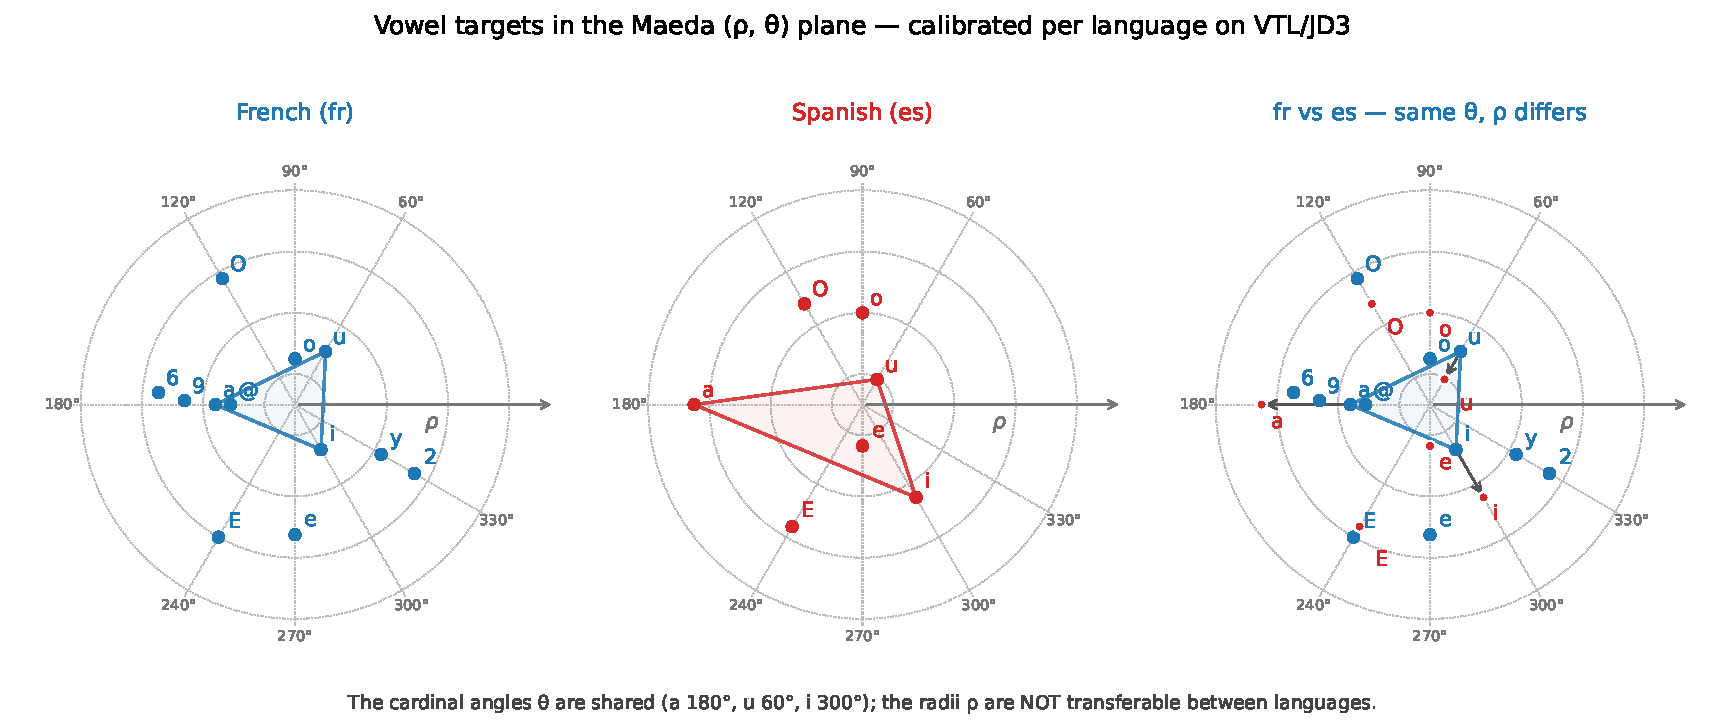
\includegraphics[width=\textwidth]{figures/vowel_triangle.pdf}
\caption{Vowel targets of French (blue) and Spanish (red) in the
$(\rho,\theta)$ plane, read directly from the shipped language
blocks. Left/middle: each language with its a-i-u triangle. Right:
overlay --- the cardinal \emph{angles} are shared, the
\emph{radii} differ (French /i/ $\rho=0.34$ vs Spanish /i/
$\rho=0.70$ at the same $300^\circ$ spoke).}
\label{fig:triangle}
\end{figure}

\subsection{The validated lesson: targets do not transfer}

Because $\rho$ absorbs the engine/speaker transfer function
\emph{as seen from each language's reference formants}, a radius
calibrated for one language is generally wrong for another, even at
the same angle: Figure~\ref{fig:triangle} shows French /i/ and
Spanish /i/ sitting at the same spoke but at very different radii,
each matching its own language's F1/F2 reference. Copying vowel
targets between languages was tried and rejected during the original
in-situ calibration; the pipeline therefore carries one derivation per
language and refuses to guess. v1.0.9 generalizes this
lesson to the speaker axis: targets do not transfer across
speakers either, which is why the per-language overrides
were removed and every speaker now carries its own
recalibrated targets.

\subsection{Calibrating a language on the engine}

v1.0.9: these two commands are \emph{deprecated} --- vowel
targets belong to the speaker, not to the language, and
\code{calibrate} no longer writes anything. They are kept
here as historical documentation of the pre-1.0.9 behaviour.

Two commands derived $\rho$ mechanically (never by hand):

\begin{enumerate}
\item \code{python setup\_lang.py calibrate <lang>} runs
      \code{find\_best\_rho} for every vowel: it sweeps $\rho$ on
      the \emph{static} VTL transfer function (tract frozen at the
      target) and picks the radius whose LPC formants best match the
      language's reference F1/F2. This is a \emph{starting point} ---
      the gestural dynamics of real synthesis displace the formants.
\item \code{python setup\_lang.py calibrate <lang> --in-situ} then
      refines each radius through \textbf{real synthesis + LPC
      measurement}: for every vowel it sweeps $\rho$, applies the
      candidate to the live \code{VOWEL\_TARGETS}, synthesizes the
      isolated vowel through the pipeline (JD3) and keeps the radius
      whose \emph{measured} F1/F2 pass best. The selection criterion
      is deliberately the same as \code{verify}'s: first minimize the
      number of formants outside $\pm30\%$, then the maximum relative
      error (not the absolute Hz error, which over-weights F2 and
      accepts F1 collapses).
\end{enumerate}

The measured F1/F2 and the verdict are written as comments next to
each target --- the mechanical proof travels with the constants.
Anything not measured in situ is flagged \textsc{Hypoth\`ese}.

\subsection{Nasal vowels and schwa-free languages}

Nasal vowels are not separate targets: the g2p emits the oral base
plus a trailing \sampkey{\textasciitilde} (French
\emph{bon} \sampkey{bO\textasciitilde}, Portuguese \emph{p\~ao}
\sampkey{p@~w}); the syllabic trajectory engine strips the tilde
before the target lookup and extends the velum opening (VO) over the
vowel instead.

Languages without a phonological schwa (Italian, Spanish) simply have
no \sampkey{@} key in their \code{VOWEL\_TARGETS}. The engine handles
this: the closing vowel-vowel arcs of \code{syltraj} fall back to the
neutral anchor (which \emph{is} the schwa by definition) instead of
raising \code{KeyError '@'} --- a fix applied once in the engine core
(\code{syltraj.\_vv\_waypoint}) and required by every schwa-free
language.

% ===========================================================================
\section{Adding a new language}
\label{sec:newlang}
% ===========================================================================

The six built-in languages were added with exactly this recipe;
\code{tests/test\_multilang.py} is the executable checklist.

\begin{enumerate}
\item \textbf{Download the Wikipron lexicon} (master branch; pick the
      right dialect variant --- see the pitfalls in
      Section~\ref{sec:pipeline}):
\begin{verbatim}
curl -L -o vtl_synth/data/xx_lexicon.tsv \
  https://raw.githubusercontent.com/CUNY-CL/wikipron/master/\
data/scrape/tsv/<xxx_latn_YY>_broad_filtered.tsv
\end{verbatim}
      Beware: saving the GitHub \emph{page} instead of the raw file
      gives HTML; a file much smaller than the expected size is
      suspect. Write the license notice
      (\code{README\_xx\_lexicon.md}) beside it: Wikipron data are
      Wiktionary extractions under CC~BY-SA~3.0.
\item \textbf{Write \code{profiles/g2p\_xx.py}} on the three-stage
      model (lexicon $\rightarrow$ exceptions $\rightarrow$ rules)
      using the shared \code{lexicon\_loader} (\code{LexiconSpec}:
      filename, environment variable, IPA$\rightarrow$keys table,
      variant policy).
\item \textbf{Declare the vowel inventory} in
      \code{profiles/language\_vowel\_sets.py}: one entry per vowel
      with the reference F1/F2 for a male speaker of the language
      (literature --- e.g.\ Quilis 1981 for es, J{\o}rgensen 1969 for
      de, Ferrero et al.\ 1978 for it, Delgado-Martins 1999 /
      Escudero et al.\ 2009 for pt), the cardinal angle, and a
      description; give the cardinal corners (\emph{a, i, u}) and the
      schwa key (\texttt{None} if the language has none).
\item \textbf{Register a \code{LangProfile}} in
      \code{profiles/setlang.py}: g2p callable, F0 contour with its
      literature reference, default timings (state that they are
      hypotheses), notation aliases for the language's graphemes.
\item \textbf{Install and calibrate}:
\begin{verbatim}
python setup_lang.py install --lang xx
python setup_lang.py calibrate xx --in-situ
python setup_lang.py verify
\end{verbatim}
      Then freeze the calibrated block as the language's fragment in
      \code{lang\_blocks/blocks.py} (measured F1/F2 in comments;
      \textsc{Hypoth\`ese} flags where the LPC chain could not
      measure). Adjust \code{VOWEL\_EFFORT\_GAIN} after listening
      (close vowels typically need 1.3--1.5).
\item \textbf{Extend the tests}: deterministic g2p batteries
      (rules path with the lexicon variable pointed at a missing
      file, and lexicon path with the real TSV), a
      \code{VOWEL\_SETS} inventory test, and --- for the ambitious
      --- a slow in-situ verify test on the model of
      \code{test\_setlang\_\allowbreak switch\_and\_\allowbreak
      verify\_es}.
\end{enumerate}

% ===========================================================================
\section{Licensing and provenance}
\label{sec:license}
% ===========================================================================

The pipeline code (engine, COVTL model, JD3 handling) is
GPL-3.0-or-later. The language pack stacks several origins;
Table~\ref{tab:provenance} is the authoritative summary (details and
data-flow in \code{lang\_pack/ARCHITECTURE.md} and
\code{lang\_pack/LICENSE.md}).

\begin{table}[htbp]
\centering
\caption{Component provenance of the language pack.}
\label{tab:provenance}
\small
\begin{tabular}{p{0.34\textwidth}p{0.30\textwidth}p{0.28\textwidth}}
\toprule
component & origin & license / citation \\
\midrule
COVTL engine, JD3 speaker, \code{vtl\_binaries/} & covtl-pipeline
(vtl-pipeline reference) & GPL-3.0-or-later; JD3 and binaries
untouched \\
English g2p (CMUdict) & CMUdict & public domain / BSD-like; source
credited \\
g2p fr/es/de/it/pt, lexicon loader, profiles, blocks & written for
this repository & GPL-3.0-or-later \\
Pronunciation lexicons \code{xx\_lexicon.tsv} & Wikipron
(CUNY-CL/wikipron), extracted from the English Wiktionary &
CC~BY-SA~3.0 (share-alike); keep the \code{README\_xx\_lexicon.md}
notices \\
Reference formants & Fant 1973; Peterson \& Barney 1952; Quilis
1981; J{\o}rgensen 1969; Ferrero et al.\ 1978; Delgado-Martins 1999;
Escudero et al.\ 2009 & academic citation \\
Prosodic contours & Jun \& Fougeron 2002; Face 2003; Grice et al.\
2005; Avesani 1995; Frota 2000; Beckman \& Ayers 1997 (ToBI) &
academic citation \\
\bottomrule
\end{tabular}
\end{table}

\textbf{Distribution.} GPL-3.0-or-later covers the code; the Wikipron
TSV data are CC~BY-SA~3.0: redistribution must keep the attribution
notices and share the data alike (compatible with the GPL for the
distribution of the whole). Local research use carries no formality.
If the TSV size is a problem for a repository, do not commit them ---
the curl commands of Section~\ref{sec:newlang} rebuild them, and the
g2p degrades gracefully to rules alone.

\paragraph{Provenance boundary.} Everything in the language pack
originates from the sources listed in the license file and from no
other program or dataset; nothing else may be cited as a component,
origin or dependency. The only binaries involved are the
VTL 2.3/2.4 \code{vtl\_binaries/} and the JD3 speaker --- nothing
else.

% ===========================================================================
\section{Troubleshooting}
\label{sec:trouble}
% ===========================================================================

\subsection{Windows: console encoding (\code{kOR.@} symptom)}

\textbf{Symptom.} On Windows, accented text passed to the synthesizer
comes out wrong: \emph{cor\'ee} is decoded with the active OEM code
page, the UTF-8 bytes are mis-combined (mojibake of the
``cor\~A(c)ee'' kind), and the French g2p then emits engine keys from
the corrupted string --- the canonical observed output being
\sampkey{kOR.@} instead of \sampkey{koRe.@} in the demo phrase.

\textbf{Fix --- two invariants.}
\begin{enumerate}
\item \code{chcp 65001 >nul} must be the first command of any
      Windows batch that passes text to the pipeline (it switches the
      console to UTF-8). It is the first line after \code{@echo off}
      in \code{install\_lang.bat} and \code{launch.bat}; keep it
      there when you edit those files.
\item The \code{.bat} files themselves must stay encoded
      \textbf{UTF-8 without BOM} (a BOM breaks the first line at
      execution).
\end{enumerate}
If you see the \sampkey{kOR.@}-style symptom, one of the two
invariants was broken (typically the file was re-saved by an editor
that added a BOM or moved the \code{chcp} line). Reading this
subsection is the one-minute diagnosis.

\subsection{\code{KeyError '@'} (schwa-free languages)}

The trajectory engine used to look up the schwa target when routing
closing vowel-vowel arcs; Italian and Spanish have no
\sampkey{@}. The engine now falls back to the neutral anchor
(Section~\ref{sec:geometry}). If you ever see \code{KeyError '@'}
again, a custom language block is missing the neutral fallback ---
check that \code{syltraj.\_vv\_waypoint} still contains it.

\subsection{LPC instability on front-rounded vowels}

The \code{verify} LPC chain can return noticeably different F2 values
between runs on close front-rounded vowels and the German schwa (the
shipped blocks document a 1484 vs 896~Hz bimodal measurement at an
identical target). If a verdict flips between two runs of
\code{verify}, re-run once before drawing conclusions; treat
borderline vowels (within a few percent of the $\pm30\%$ edge) as
measurement noise, per the comments in the language blocks.

\subsection{Restore a pristine tree}

\begin{verbatim}
    python setup_lang.py restore           # original files back
    python setup_lang.py restore --purge   # + remove pack modules
\end{verbatim}

\code{restore} puts back the backed-up \code{constants.py},
\code{pipeline.py} and \code{utils/\_\_init\_\_.py} (the
\code{.bak} files are kept for later reinstalls); \code{--purge}
additionally deletes the installed language modules (those listed in
the module manifest) and the lexicon files the install itself brought
in. Repository-tracked lexicons and anything you modified are never
deleted. After a purge the tree is byte-identical to a fresh clone,
and \code{install} brings the pack back at any time.

\subsection{Verify reports far fewer vowels than expected}

Check that the active language is what you think
(\code{python setup\_lang.py show} --- every command prints it), that
the VTL bindings import (\code{python -c "import
vocaltractlab\_cython"}), that the JD3 speaker is present in
\code{vtl\_synth/data/vtl\_binaries/}, and that the LANG~SECTION of
\code{constants.py} still carries both markers. A
\code{Bilan} line consistent with Table~\ref{tab:verdicts} means the
installation is healthy whatever the individual deviations say.

\end{document}
